\documentclass[a4paper, 12pt,oneside]{article} 
%\documentclass[a4paper, 12pt,oneside,draft]{article} 
\usepackage{preamble}
\usepackage{pythonhighlight}

%--------------------- ACTUAL FILE ---------------------- %
\begin{document} 
%%%
	%\setcounter{page}{1}
	\begin{center}
	    \Large
	    \textbf{HMC : When is it worth over RWMC ?} 
	    \vspace{0.4cm}
	    \large

		Course : Stochastic Simulation \\
	    Students : Aude Maier \& Tara Fjellman \\
	    \small{Fall 2024}
	\end{center}

	\section{Introduction}
	\section{Core Theory}
		\subsection{RWMC}
		\subsection{HMC}
			\subsubsection{The Algorithm}
			A common shortfall of the simple random walk Metropolis proposal in the Metropolis-Hastings algorithm is the slow exploration rate of the state space. Much effort has been devoted in recent years to devise proposals with more efficient exploration rates (i.e "distant" proposals). One idea borrowed from physics, which, can be applied to most problems with continuous state space, is to introduce a "fictitious" Hamiltonian dynamics and "fictitious" momentum variables.

			We recall that a Hamiltonian dynamical system is characterized by a Hamiltonian function $H$ : $\mathbb{R}^d \times \mathbb{R}^d \rightarrow \mathbb{R}, H=H(q, p)$, that is conserved during dynamics. Here $q=\left(q_1, \ldots, q_d\right)$ denotes the position vector and $p=\left(p_1, \ldots, p_d\right)$ denotes the momentum vector. The Hamiltonian dynamics is governed by the equations
			
			$$
			\begin{aligned}
			\frac{d q_i}{d t} & =\frac{\partial H}{\partial p_i} \\
			\frac{d p_i}{d t} & =-\frac{\partial H}{\partial q_i}
			\end{aligned}
			$$
			
			for $i=1, \ldots, d$. In general, the above equation can be understood as a conservation of the total energy of a system in time.
			Hamiltonian Monte Carlo takes inspiration from the previous physical system in order to construct a Markov Chain Monte Carlo algorithm with a given invariant density $\pi(q)$ on the position variables $\left(q_1, \ldots, q_d\right)$. To do so, we introduce the potential energy $U(q)=-\log \pi(q)$, a kinetic energy $K(p)=\sum_{i=1}^d \frac{p_i^2}{2 m_i}$, for some mass parameters $m_i, i=1, \ldots, d$, and the Hamiltonian $H(q, p)=U(q)+K(p)$. Having introduced these functions, we can then simulate a Markov chain in which each iteration re-samples the momentum, evolves the Hamiltonian system for a certain time, and then performs a Metropolis-type acceptance-rejection step on the new position vector. More concretely, we consider the so-called Gibbs distribution, given by

			$$
			G(q, p)=\frac{1}{Z} \exp (-H(p, q))
			$$
			
			where $Z$ is the (unknown) normalizing constant. Notice that such a Gibbs distribution naturally factorizes as:

			$$
			G(q, p)=\frac{1}{\tilde{Z}} \exp (-U(q)) \frac{1}{\prod_{i=1}^d \sqrt{2 \pi m_i}} \exp (-K(p))
			$$
			
			where $\frac{1}{Z} \exp (-U(q))$ is the probability density we are interested in sampling from, whereas $\frac{\exp (-K(p))}{\Pi_{i=1}^d \sqrt{2 \pi m_i}}$ is a multivariate Gaussian distribution $N(0, M)$ with $M=\operatorname{diag}\left(m_1, \ldots, m_d\right)$. Given the state $q^n$ at iteration $n$, the idea of the algorithm is then to sample a momentum vector $p^n$ from $N(0, M)$, and compute $H\left(q^n, p^n\right)$. The Hamiltonian system is then evolved starting from $q(0)=q^n, p(0)=p^n$, on a time interval [0,T] using equations (1), and (2) for some arbitrary final time $T$, to obtain $(q(T), p(T))$, where, in general, $q(T) \neq q(0)$. This state is then taken as the proposal state in a Metropolis-Hastings step to generate the new state $q^{n+1}$. For many problems of modern relevance, it is not possible to compute the dynamics exactly and numerical discretization is needed. A convenient time discretization scheme is the Verlet's method: the time interval $[0, T]$ is divided into $N_t$ intervals of size $\epsilon>0$ and for each particle $i$ the position $q_i$ and momemtum $p_i$ are updated as follows
			
			$$
			\begin{aligned}
			& p_i(t+\epsilon / 2)=p_i(t)-(\epsilon / 2) \frac{\partial U(q(t))}{\partial q_i} \\
			& q_i(t+\epsilon)=q_i(t)+\epsilon \frac{p_i(t+\epsilon / 2)}{m_i} \\
			& p_i(t+\epsilon)=p_i(t+\epsilon / 2)-(\epsilon / 2) \frac{\partial U(q(t+\epsilon))}{\partial q_i}
			\end{aligned}
			$$
			
			
			The main steps of the Hamiltonian Monte Carlo algorithm using Verlet's method are outlined in Algorithm 1. There, $N$ is the length of the chain, $\epsilon$ the time step in Verlet's method, and $T$ the final integration time.
			\subsubsection{Acceptance Rate}
			To explore how the acceptance rate behaves in HMC, we must consider the quantity \newline $\exp \left[U\left(q^n\right)+K\left(p^n\right)-U\left(q^*\right)-K\left(p^*\right)\right]$ which appears in the expression for $\alpha$ in the Metropolis-Hastings acceptance probability. Using the definition $H(q, p)=U(q)+K(p)$ we can write this quantity as:
			\begin{gather}
				\exp \left(U\left(q^n\right)+K\left(p^n\right)-U\left(q^*\right)-K\left(p^*\right)\right) = \exp \left[H\left(q^n, p^n\right)-H\left(q^* p^*\right)\right].
				\label{eq:HMC-acceptance-rate} 
			\end{gather}
			Since the Hamiltonian is conserved under the Hamiltonian dynamics :
			\begin{align}
			\frac{d H}{d t}=&\sum_i \frac{\partial H}{\partial p_i} \frac{d p_i}{d t}+\sum \frac{\partial H}{\partial q_i} \frac{\partial q_i}{d t} \\
			=&-\sum_i \frac{\partial H}{\partial p_i} \frac{\partial H}{\partial q_i}+\sum_i \frac{\partial H}{\partial q_i} \frac{\partial H_i}{\partial p_i} = 0,
			\end{align}
			we find by using this in \ref{eq:HMC-acceptance-rate} that if integration is exact, the acceptance rate is always 1.

			Under the assumption that the Hamiltonian dynamics is discretised, conservation is there in the best case on average. This implies the acceptance rate will be less than 1. 
			\subsubsection{Convergence to Target Distribution}
			\paragraph{Gibbs distribution invariance}
			Under the assumption that there is no numerical error, we want to prove that the Gibbs measure is invariant for the chain generated by the hamiltonian dynamics.
	
			This is equivalent to saying that the Gibbs measure $\pi$ is the same before and after an evolution of $t$ seconds from the hamiltonian dynamics. 
			To prove this we first introduce hamiltonian dynamics operators $\phi,\Phi$ acting respectively on the phase space and the Gibbs measure : $\phi_t(q_s,p_s)=(q_{s+t},p_{s+t});\Phi_t[\pi_s]=\pi_{t+s}\quad \forall t\in\mathbb{R}$.
			The statement we want to prove can then be expressed as 
			\begin{gather}
				\Phi_t[\pi_s](D)=\pi_{s+t}(D)\quad \forall D\in\mathcal{B}(\Omega),\forall s,t\in\mathbb{R},
				%P(T_t(q,p)\in D_s)=
				%P((q,p)\in T_{-t}(D_s))=
				%P((q,p)\in D_s)=\pi(D_s),
				%P((q,p))=\int_{\Omega} K((q,p),D_s) G(q,p) \ dq dp=\pi(T_t[D_s]),
			\end{gather}
			with $\Omega$ the phase space.
	
			We can now write the left hand side of the equation as
			\begin{align}
				\Phi_t[\pi_s](D)&=\int_D \pi_{s+t}(q,p)\ dqdp \\
					&=\int_{\phi_{-t}(D)}\pi_{s}(q,p)\ dqdp \\
					&=\pi_s(\phi_{-t}(D)).
			\end{align}
			The final result is obtained using the fact that volumes in phase space are preserved by the hamiltonian dynamics (in conservative systems). This result is known as Liouville's theorem, but is mentioned as theorems 2.3 in [cite].
			%K:\Omega \times D\to [0,1]$ the transition kernel of the chain, $G(q,p)$ the Gibbs distribution, and $T_t[\cdot]$ the hamiltonian time evolution operator defined by $T[(q_s,p_s)]=(q_{s+t},p_{s+t})$.
	
			This implies specifically that $q_k\sim\pi$ for all $k\in\mathbb{N}$ if $q_0\sim \pi$. 
	
			If the dynamics is discretised with the Velocity Verlet algorithm, the volume in phase space is preserved up to a small error, which is why the algorithm is used in practice [cite wikipedia].
	\section{Exploring a 2D example}
		\subsection{Context}
		In this section we explore the performance of the presented algorithms on a 2D example. The target distribution is taken as $f_1(q_1,q_2)=e^{-\alpha(q_1^2+q_2^2-0.25)^2}$, with $\alpha>0$ a parameter. This unormalised density is represented in figure \ref{fig:alpha-density} for two different values of $\alpha$.
        \begin{figure}[htb]
            \centering
                \vspace{0em}
                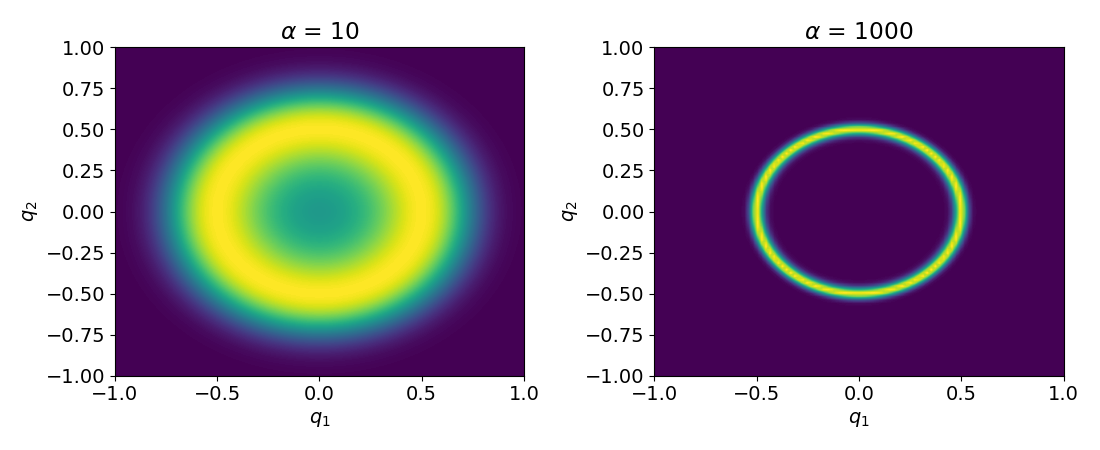
\includegraphics[width=0.9\textwidth]{alpha_density}
                \caption{Density considered in this section for two different values of $\alpha$.}
                \label{fig:alpha-density}
        \end{figure}
		As it can be seen, the density has the shape of a doughnot and $\alpha$ controls its thickness. We expect the $\alpha=1000$ case to be more difficult to sample from than the $\alpha=10$ case, as the density is more localised.
		\subsection{RWMC Solution}
			As seen previously, the RWMC algorithms only depends on the step size. To find the best RWMC sampler we therefore explore the impact of the step size on performance. 
			
			Here and in the following, We decide to quantify performance throught the computation of a similarity based on the Jensen-Shannon divergence. This choice allows us to feed in a discretised version of $f_1$ (which we can normalise) and the empirical distribution of the samples generated by the algorithm, and get a similarity measure between the two.

			The similarities associated to 3000 samples for the different step sizes are presented in figure \ref{fig:rwmc-scan}.
			\begin{figure}[htb]
				\centering
					\vspace{0em}
					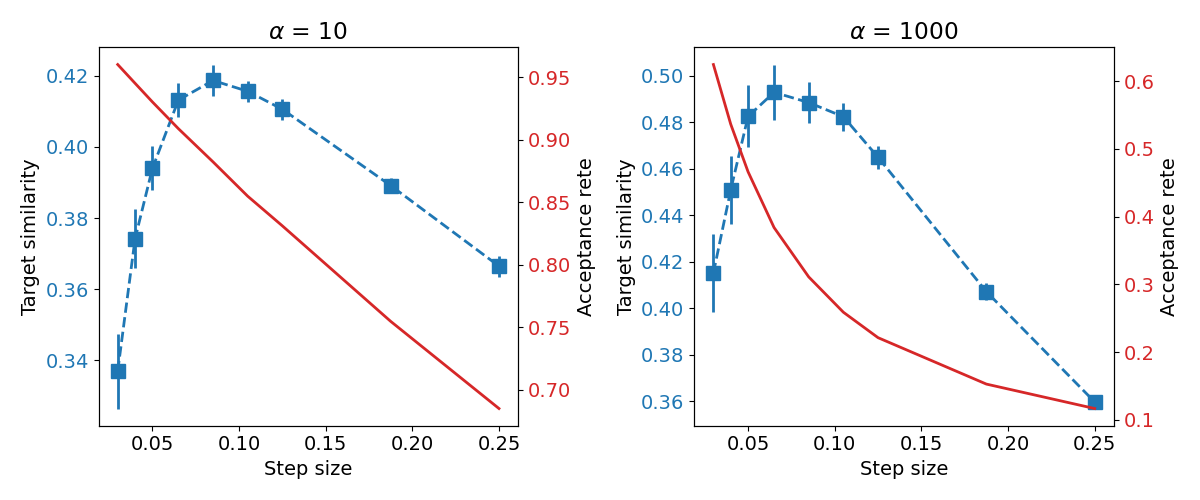
\includegraphics[width=0.95\textwidth]{rwmc_scan}
					\caption{Similarity as a function of RWMC step size for considered values of $\alpha$.}
					\label{fig:rwmc-scan}
			\end{figure}

			- both plots display a peak for a step size in the centre of the range considered (around 8.5$\times 10^{-2}$ and 6.5$\times 10^{-2}$ for $\alpha=10$ and $\alpha=1000$ respectively). This is expected as the step size is a tuning parameter that should be chosen to match the scale of the target distribution.
			- the peak is sharper (espescially on the right) for the $\alpha=1000$ case, which is consistent with the fact that the density is more localised. 
			- the value of the similarity is in all cases smaller than .5, which means that 3000 samples are too few to accurately estimate the target distribution. The value is higher in the $\alpha=1000$ case, which can at first look surprising. Indeed, this case is meant to be harder than the $\alpha=10$ one, but the fact that the density is more localised for $\alpha=1000$ actually means that there are fewer places where the estimate and the target can differ, which can lead to a better similarity. It is therefore most important to consider the relative values of the similarities for the different step sizes, rather than the absolute values.
			- looking at acceptance rate, we see that they are of course monotonically deacreasing with step size. This means that the obtimal value corresponds with the best exploration-acceptance rate trade-off. The acceptance rate is higher and decreases slower for the $\alpha=10$ case, which is consistent with the fact that the density is more spread out. The acceptance rate of the $\alpha=1000$ case associated to the best step size is still around .55, which suggests that this case is still quite easy to sample from. 
		\subsection{HMC Solution}
			\begin{wrapfigure}[18]{r}{0.6\textwidth}
				\centering
					\vspace{-2em}
					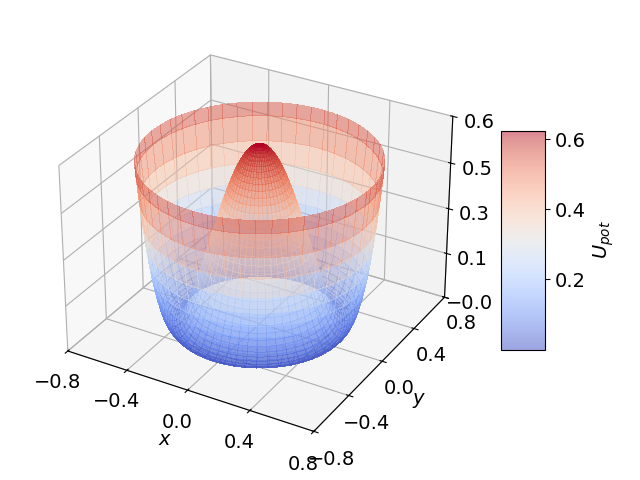
\includegraphics[width=0.57\textwidth]{U_pot_alpha=10}
					\caption{Potential energy landscape associated to HMC algorithm for $\alpha=10$. Version for $\alpha=1000$ is identical, except scales are scaled by a factor of 100.}
					\label{fig:U-pot-alpha=10}
			\end{wrapfigure}
			Before exploring the impact of the different parameters of the HMC algorithm, we first present the potential energy landscape associated to the algorithm for this specific problem. The landscape is presented in figure \ref{fig:U-pot-alpha=10}. 
			The landscape has polar symmetry, meaning the trajectories will be some sort of symmetric oscillations. It has global minima at a radius of $\sqrt{0.25}=0.5$ away from the centre and a local maxima at the centre. The only difference in the landscape for $\alpha=1000$ w.r.t. the $\alpha=10$ one is the scale of the potential. This means that the $\alpha=1000$ will give rise to stronger potential forces, which translates the fact that the density is more localised. 
			\subsubsection{Impact of Integration Time}
			The first parameter we explore is the integration time. For this parameter, we expect the optimal value to be the one that allows the sampler to explore the whole space, without being excessively long (as it would slow down sampling).
			The similarities associated to 3000 samples for the different integration times are presented in figure \ref{fig:t-scan}.
			\begin{figure}[htb]
				\centering
					\vspace{0em}
					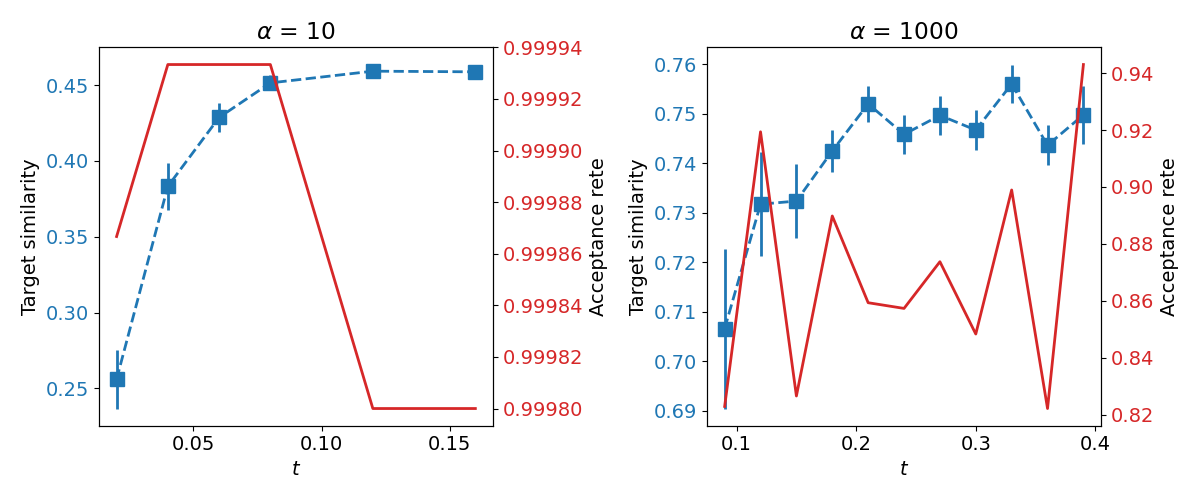
\includegraphics[width=0.95\textwidth]{t_scan}
					\caption{Similarity as a function of HMC integration time for considered values of $\alpha$.}
					\label{fig:t-scan}
			\end{figure}
			From a qualitative point of view, the behaviour is the same for both settings : similarity increases as a function of $t$ untill a plateau is reached. Looking more closely, we notice that the curve is more noisy for the $\alpha=1000$ case. This might be due to the smaller characteristic time of the dynamics, which makes the particle .... [FILL]
			- the plateau is reached quicker for the $\alpha=10$ case, probably because the forces are stronger and the sampler can explore the space more quickly.
			For the $\alpha=10$ case, $t=8$ seems to strike a good balance for the mentionned trade-off. In the $t=1000$ case ...[FILL] 
			\subsection{Impact of $\Delta t$}
			The next parameter we explore is the time step. This parameter is important as it controls the accuracy of the integration. The goal is to find the largest time step thata allows for accurate integration, as this will speed up the sampler while allowing it to accept proposals frequently.

			The similarities associated to 3000 samples for the different time steps are presented in figure \ref{fig:dt-scan}.
			\begin{figure}[htb]
				\centering
					\vspace{0em}
					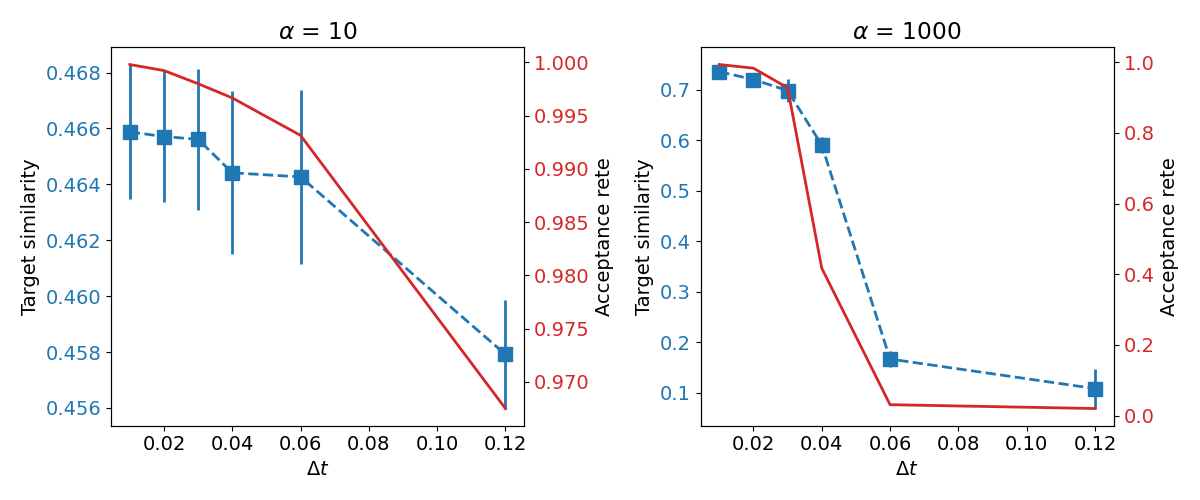
\includegraphics[width=0.95\textwidth]{dt_scan}
					\caption{Similarity as a function of HMC time step for considered values of $\alpha$.}
					\label{fig:dt-scan}
			\end{figure}
			The first characteristic feature the two plots share is the monotonous behaviour of target-similarity and acceptance rate. Indeed, as mentionned before, by making $\Delta t$ grow, the simulation does not exactly leave the Hamiltonian invariant, and therefore makes the acceptance rate decrease. This in turn affects the similarity, as the obtained samples are less diverse and represent the target distribution less precisely.  
			Looking more closely though, we notice the speed of decrease is really different : it is much quicker and of bigger scale for $\alpha=1000$ (we basically reach 0 for the acceptance rate when $\Delta t=6\times 10^{-2}$). This is due to the characteristic time being shorter, and therefore requiring finer resolution. Indeed, one can only go up to $\Delta t=3\times 10^{-2}$ before really suffering in terms of performance, while for $\alpha=10$ good performance is mantained in term of target similarity even when a single timestep of size $t$ is taken (look at the scale of the vertical axis). This makes sense since the obtained algorithm is still some sort of upgraded version of RWMC where the general direction of the step is choosen smartly and RWMC already performed well over quite a broad domain of step sizes.   
			\subsection{Impact of Mass Scale}
			We now turn to analysing the impact of the mass. We split this in terms of the mass scale and the mass symmetry. We do not consider the impact of off-diagonal terms as this would make the report too long. 

			What we expect to see is that the mass scale will control the speed of the dynamics (by affecting the particle's inertia).
			The similarities associated to 3000 samples for the different mass scales are presented in \ref{fig:mass-scan}.
			\begin{figure}[htb]
				\centering
					\vspace{0em}
					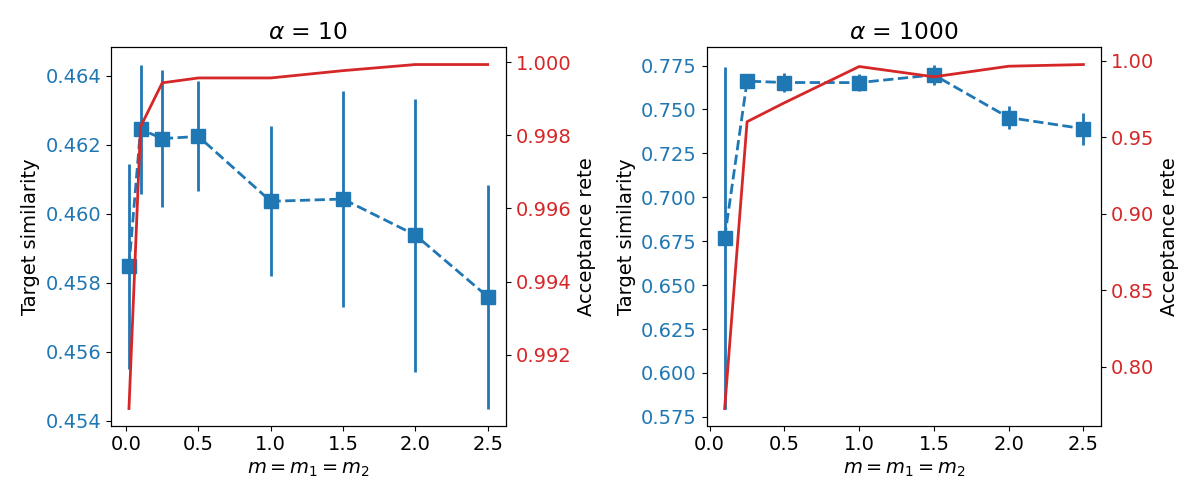
\includegraphics[width=0.95\textwidth]{mass_scan}
					\caption{Similarity as a function of HMC mass scale for considered values of $\alpha$.}
					\label{fig:mass-scan}
			\end{figure}
			- In this case, both plots look qualitatively similar : both the acceptance rate and the similarity admit a global maxima at some value of the mass scale, and worsen on both sides of it. in both cases the acceptance rate reaches zero for a value of the order twice the optimal value.  
			- bigger masses are better for alpha =1000
			- reason for decrease on both end in terms of poor integration (citing GPT for stiff systems being harder)
			- 
			\subsection{Impact of Mass Symmetry}
			What we expect to see is that mass symmetry will control the isotropy/anisotropy of the trajectories. Indeed, if masses are different, the particle will have different inertia in different directions, which will affect the shape of the trajectories : in some direction the particle will react quickly to forces, while in others it will be more inert. We try to gain insight into this with help of  \ref{fig:mass-sym}, in which the similarities associated to 3000 samples for both symmetric and asymmetric masses are represented.
			\begin{figure}[htb]
				\centering
					\vspace{0em}
					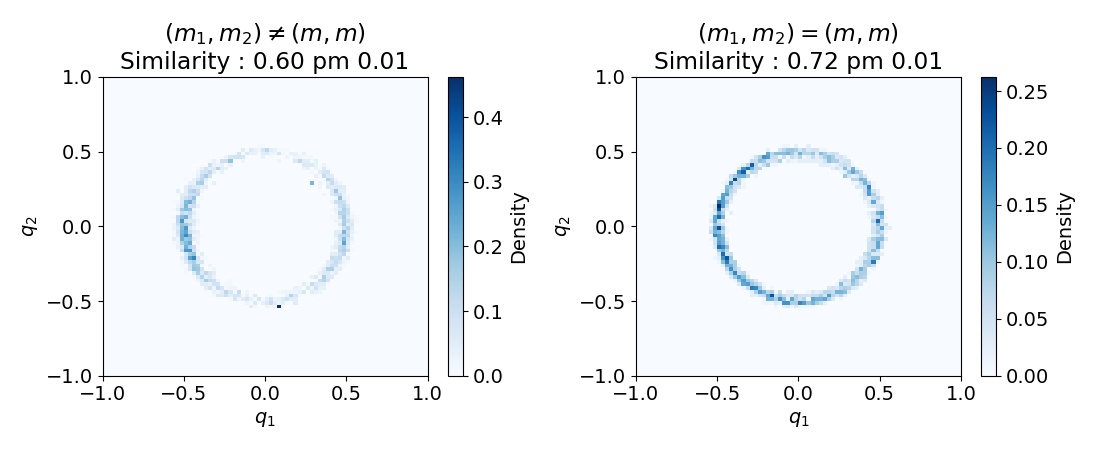
\includegraphics[width=0.95\textwidth]{mass_sym}
					\caption{Similarity for HMC samplers with asymmetric and symmetric masses for $\alpha=1000$.}
					\label{fig:mass-sym}
			\end{figure}
			- A first look at the plot shows that the similarity is better for the symmetric mass case. This makes sense given the target distribution (and therefore potential landscape) is isotropic. We would expect this to change if the distribution was anisotropic. If the main axis of motion were to not be orthogonal, we would expect to find an advantage in properly choosing off-diagonal terms for the mass. 
			- more precisely, in the anisotropic case it can be seen that the left and right areas of the distributions are sampled more than the top and bottom ones. This seems to be a consequence of the fact that in that example $m_1>m_2$, and therefore the particle's inertia is stronger along the horizontal axis than the vertical one. 
			\subsection{Comment on interractions between parameters}
		\subsection{Comparison and Sample-Size Evolution}
		- finding global optimal choice of parameters without doing a grid-search (which is untractable in high dimensions), is not easy. This is due to interdependence of the parameters. Indeed .....
		- in practice we looked for a way to find ``good enough'' parameters easily. The way we came up with was the following : 
		....

		....

		Applying this method, it is interesting to compare the obtained results with those of the step-size-optimised RWMC 
		\begin{figure}[htb]
			\centering
				\vspace{0em}
				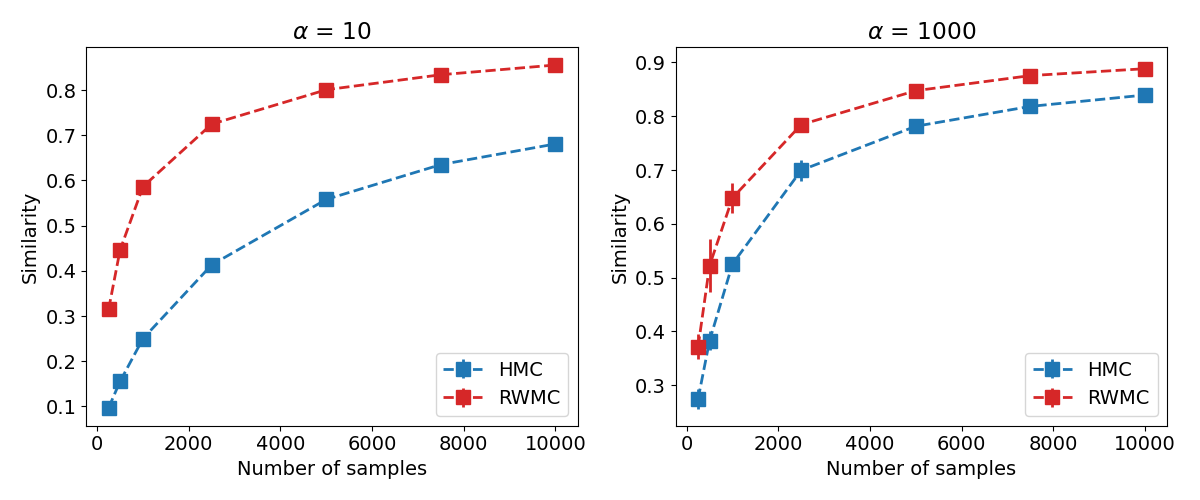
\includegraphics[width=0.9\textwidth]{nsamples_evolution}
				\caption{Similarity as a function of sample-size for RWMC and HMC samplers and considered values of $\alpha$. The sample-size represented on the x axis is that associated to the HMC sampler. The associated RWMC sample-size is obtained by matching the number of function evalutations of the HMC sampler.}
				\label{fig:nsamples-evolution}
		\end{figure}
		\lipsum[1]
	\section{US Birthweight Data}
		\subsection{HMC Solution}
		\subsection{RWMC Solution}
	\section{Section ...}
	\section{Conclusion}
	\section*{Aknowledgements}
	\section*{References}
	\appendix
		\section{Commented Code Snippet}\label{appendix:commented-code-snippet}
			[cite stack exchange for format]
			\begin{python}
			if transactions: Transaction.create_transactions() # if transactions = "true"
			node.generate_emptyState() # empty state for all nodes
			S.initial_events() # initiate initial events to start with

			while not queue.isEmpty() and clock <= targetTime:
				next_e = queue.get_next_event()
				clock = next_e.time # move clock to the time of the event
				Event.execute_event(next_e)
				Queue.remove_event(next_e)

			print results
			\end{python}
		\section{Rejection Sampling Attempt}\label{appendix:rejection-sampling-attempt}
		As an alternative to HMC we consider rejection sampling. We therefore want to find a function $g(q)$ and a constant $C$ such that the following inequality holds for all $q$:
		\begin{equation}
			\tilde{f}(q) = e^{q^TX^T(y-1_{n})}e^{-1_{n}^T \log[1+\exp(-x_i^Tq)]_{n\times 1}}e^{-\frac{1}{2}q^T\Sigma^{-1} q} \leq Cg(q),
		\end{equation}
		where we have denoted $\Sigma=\text{Diag}(\sigma_1^2,...,\sigma_p^2)$.
		Given that 
		\begin{equation}
			\log[1+\exp(-x_i^Tq)] \le \log(2) - x_i^Tq,
		\end{equation}
		\begin{equation}
			e^{-\sum_i \log[1+\exp(-x_i^Tq)]} = \prod_i \frac{1}{1+\exp(-x_i^Tq)}<1,
		\end{equation}
		we can simplify the problem to finding a function $g(q)$ such that
		\begin{equation}
			\tilde{f}(q) \le 2^{-n}e^{-q^TX^T 1_n} e^{q^TX^T(y-1_{n})}e^{-\frac{1}{2}q^T\Sigma^{-1} q} = 2^{-n}e^{q^Tb}e^{-\frac{1}{2}q^T\Sigma^{-1} q}
			=: Cg(q),
		\end{equation}
		with $b=X^T(y-2_{n})$. 
	
		By completing the square in the exponent of $Cg(q)$, we can write it in terms of a Multivariate Gaussian distribution with mean $\mu=\Sigma b$ and covariance $\Sigma$. Indeed : 
		% TO DO : change into a double equality going from Cg(q) to clean expression in terms of completed square
		\begin{gather}
			%e^{q^Tb}e^{-\frac{1}{2}q^T\Sigma^{-1} q} = 
			e^{-\frac{1}{2}(q-\mu)^T\Sigma^{-1} (q-\mu)} =
			e^{-\frac{1}{2}\mu^T\Sigma^{-1}\mu}
			e^{q^T\Sigma^{-1}\mu}
			e^{-\frac{1}{2}q^T\Sigma^{-1} q} \\
			\implies \tilde{f}(q) \le 2^{-n}e^{\frac{1}{2}\mu^T\Sigma^{-1} \mu}e^{-\frac{1}{2}(q-\mu)^T\Sigma^{-1}(q-\mu)}.
		\end{gather}
		Using now the normalisation constant of the Multivariate Gaussian distribution 
		\begin{gather}
			\sqrt{(2\pi)^p|\Sigma|}=\int_{\mathbb{R}^p}e^{-\frac{1}{2}(q-\mu)^T\Sigma^{-1}(q-\mu)}\ dq,
		\end{gather} 
		we can define $g$ and $C$ as 
		\begin{gather}
			g(q)=\frac{1}{\sqrt{(2\pi)^p|\Sigma|}}e^{-\frac{1}{2}(q-\mu)^T\Sigma^{-1}(q-\mu)}, \\
			C = 2^{-n}e^{\frac{1}{2}\mu^T\Sigma^{-1} \mu}{\sqrt{(2\pi)^p|\Sigma|}} = 2^{-n}\sqrt{(2\pi)^p|\Sigma|e^{\mu^T\Sigma^{-1} \mu}}.
		\end{gather} 
%%%
\end{document} 

